\label{sec:subdivision_euler}

The $\sqrt{3}$ subdivision scheme was introduced by
Kobbelt~\cite{sqrt3}. It takes as input a triangle mesh and
subdivide each facet into three triangles by splitting it at its
centroid. Next, all edges of the initial mesh are flipped so that they
join two adjacent centroids. Finally, each initial vertex is replaced
by a barycentric combination of its neighbors. An example of one step
of the $\sqrt{3}$ subdivision scheme is shown in
Fig.\ref{fig:sqrt3_basic}, and an example of several steps is shown in
Fig.\ref{fig:sqrt3}.

% sqrt3 subdivision (basic)

\begin{figure}[htb]
    \centering{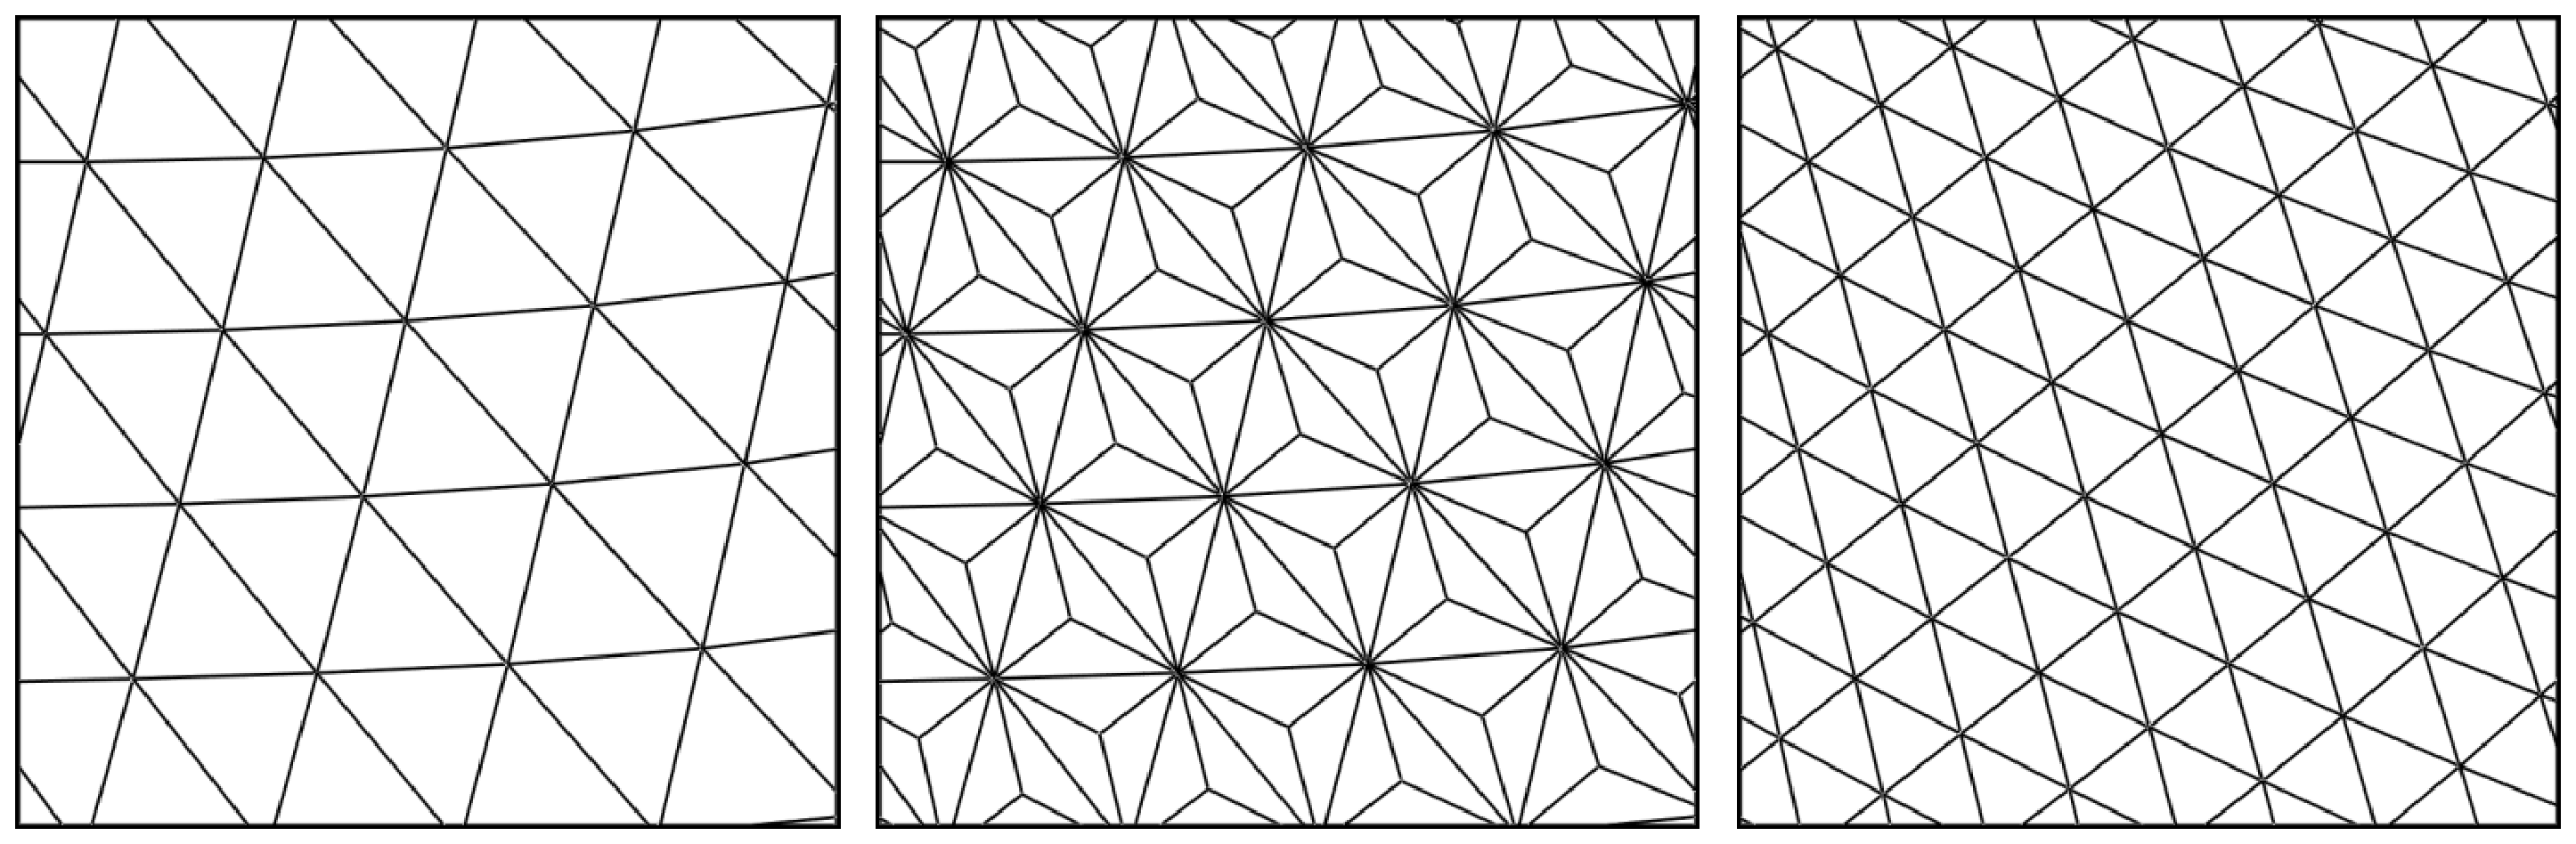
\includegraphics[width=10.0cm]{figs/sqrt3_basic}}
    \caption{The $\sqrt{3}$-Subdivision scheme is decomposed as
             a set of Euler operators: face splits and edge flips.}
    \label{fig:sqrt3_basic}
\end{figure}

%{ 

%\scriptsize
%\begin{verbatim}



%\end{verbatim}
%}

% sqrt3 subdivision 

\begin{figure}[htb]
    \centering{\includegraphics[width=10.0cm]{figs/sqrt3}}
    \caption{$\sqrt{3}$ subdivision of the mannequin mesh.}
    \label{fig:sqrt3}
\end{figure}
